\documentclass[10pt,letterpaper]{article}
\usepackage[margin=0.78in]{geometry}
\usepackage[T1]{fontenc}
\usepackage{lmodern,microtype,graphicx,booktabs,tabularx,amsmath,amssymb,xcolor,fancyhdr,enumitem}
\usepackage[hyphens]{url}
\usepackage[colorlinks=true,linkcolor=teal,urlcolor=teal]{hyperref}
\definecolor{ink}{HTML}{243447}\definecolor{teal}{HTML}{006B72}
\setlength{\parindent}{0pt}\setlength{\parskip}{6pt}\setlist{nosep,leftmargin=1.5em}
\pagestyle{fancy}\fancyhf{}\fancyhead[L]{\small Denominators and state fatality comparisons}\fancyhead[R]{\small Independent study 19}\fancyfoot[C]{\thepage}\setlength{\headheight}{14pt}
\hypersetup{pdftitle={Denominators and state fatality comparisons},pdfauthor={Independent research program},pdfsubject={Published aggregate measurement sensitivity; not individual risk or causal policy evaluation}}
\begin{document}\color{ink}
{\LARGE\bfseries Denominators and state fatality comparisons\par}
{\large Exact counts, rounded road-user shares and different questions\par}
\textbf{Independent research study 19}\hfill29 October 2026\\
AI-assisted analysis and manuscript. Not peer reviewed or accepted for formal publication.

\section*{Decision and verified finding}
State traffic-fatality rankings depend on what is placed below the same count. Population, licensed drivers and vehicle miles describe different reference quantities. They should not be treated as interchangeable measures of individual road-user risk.

Using the fixed 2023 NHTSA State Traffic Data report, population versus vehicle-mile denominators reverse 222 of 1,275 state-pair orderings (17.4\%). Only two states are shared by their five highest-rate sets; six are shared by their ten highest-rate sets. The largest movement is the District of Columbia, from rank 47 under population to rank 26 under vehicle miles. Rank 1 denotes higher recorded fatality intensity, not a causal judgment of a jurisdiction's safety.

\begin{center}\begin{tabularx}{\linewidth}{Xr}\toprule
Fixed 2023 all-fatality comparison & Measured value\\\midrule
States and District of Columbia & 51\\
Strict reversed pairs, population versus VMT & 222 / 1,275\\
Largest absolute rank movement & 21 places\\
Top-five / top-ten set overlap & 2 / 6 states\\\bottomrule
\end{tabularx}\end{center}

The source's precision also matters. The 2019 and 2021 selected person-type tables report rounded percentages, while the 2023 table additionally supplies exact subgroup counts. In a declared coarsening sensitivity, the 2023 pedalcyclist percentages guarantee only 7 of the 126 reversals observed with the supplied exact counts; 119 of those reversals fall in pairs left unresolved by the ranges. We retain both representations and recommend using exact counts when available.

\textbf{Practical recommendation.} State the count, denominator, location basis, report vintage and precision together. Show alternative denominators when the interpretation depends on them. Preserve the source's exact counts and use conditional ranges for rounded shares rather than manufacturing point counts. Obtain road-user travel exposure before making individual-risk or resource-allocation claims.

\textbf{Limits.} These are three separate published Annual Report File snapshots, not latest harmonized FARS data or a prospective risk model. Fatalities occur in a state and can include nonresidents; dividing them by resident population does not estimate resident death risk. Motor-vehicle miles and licensed drivers are not pedestrian or cyclist person-distance. Rounded-display ranges are conditional arithmetic scenarios, not statistical confidence intervals or bounds on true exposure. No causal policy, clinical, individual-safety, legal-compliance or realized-benefit claim is made.

\clearpage
\section*{1. Fixed source panel and boundaries}
We use Tables 1 and 7 from NHTSA's State Traffic Data reports for 2019, 2021 and 2023 [1--3]. Each report describes its own FARS Annual Report File (ARF), with population attributed to the Census Bureau and licensed-driver/VMT figures to the Federal Highway Administration (FHWA). We preserve the report snapshots instead of blending their cells with later revised online totals.

\begin{center}\begin{tabular}{llrr}\toprule
Report year & Publication & U.S. fatalities & Eligible state rows\\\midrule
2019 & October 2021; DOT HS 813 183 & 36,096 & 51\\
2021 & September 2023; DOT HS 813 509 & 42,939 & 51\\
2023 & August 2025; DOT HS 813 743 & 40,901 & 51\\\bottomrule
\end{tabular}\end{center}

The panel contains 153 eligible state-year rows. All 50 states and DC are retained. Each source table also includes a national accounting row and Puerto Rico; Puerto Rico is excluded from state comparisons, consistently with the reports' U.S. total definition. No state or year is selected after seeing the ranking results.

Table 1 provides total fatalities, population, licensed drivers, VMT in millions and the three corresponding displayed rates. Registered-vehicle counts/rates are excluded, including national figures attributed to copyrighted Polk/S\&P Global Mobility material. Table 7 provides total fatalities and five whole-percent person-type shares. The 2023 table also supplies counts for those five groups. Older exact subgroup counts remain missing; no percentage product is relabeled as an observed count.

\textbf{Source-schema correction before analysis.} The original six-token Table 7 gate rejected the 2023 table's added count columns. We preserved the failure and exact responses, documented a prospective schema update, selected both counts and shares, and added an exact-count comparator before computing any ranking analysis. Retrieval resumed captured responses without refreshing or overwriting them. This source-driven update did not select a result, threshold or state subset.

All three official responses were multipart bodies containing one PDF. We retained the exact response hash and separately decoded payload hash. Complete PDFs, their prose, agency artwork and source-table images remain outside Git. Only selected factual cells, source locators, hashes and original analysis are published. These are public aggregate statistics, not person-level clinical, address, crash-location or vehicle-identifier records. No blanket CC0 license or agency endorsement is asserted; the source and factual-extraction boundary are documented [6].

\textbf{Reconciliation.} Fatality, population and licensed-driver state sums match their report's national totals exactly. Summed displayed VMT exceeds the national figure by 2 million miles in 2019, 2 million in 2021 and 1 million in 2023. We retain those differences and do not rescale state denominators. Each state's reported rate passes the fixed printed-precision consistency check.

\clearpage
\section*{2. Exact rates and conditional precision ranges}
For recorded fatalities $N_s$ in state $s$ and denominator $D_s$, use $R_s=cN_s/D_s$, with $c=100{,}000$ for population/licensed drivers and $c=100$ when VMT is recorded in millions. All ranking comparisons use exact rational values. Equal rates receive midranks; fixed top-five/top-ten sets include all ties at the threshold. These shortlist sizes are illustrative conventions, not empirically optimized policy budgets.

For states $i,j$ and denominator views $a,b$, a strict reversal requires
\[
\operatorname{sign}(N_iD_{ja}-N_jD_{ia})
\operatorname{sign}(N_iD_{jb}-N_jD_{ib})=-1.
\]
Ties in either view are separate. All 1,275 pairs, all three denominator contrasts and all years are retained. The primary comparison is 2023 all-fatality population versus VMT; the others are fixed context and sensitivity analyses, not a model search. No significance test is attached to this finite panel.

\subsection*{Rounded shares}
For total $N$ and printed whole percentage $p$, retain integer subgroup counts in
\[
L=\left\lceil N\max(0,p-0.5)/100\right\rceil,\qquad
U=\left\lfloor N\min(100,p+0.5)/100\right\rfloor.
\]
Both half-percentage endpoints are included conservatively across tie-rounding conventions; we do not assert NHTSA's undisclosed rounding rule. Require nonempty intervals and the sum of all five lower counts at most $N$. Tighten each upper bound by subtracting the other four lower counts from $N$. Other/unknown person types retain a nonnegative remainder. For example, a displayed 0\% with $N=1{,}000$ permits zero through five fatalities under this closed convention; it is not proof of zero.

For a fixed display-precision sensitivity, VMT may vary by $\pm0.5$ million around its printed integer; population and licensed-driver cells stay fixed. Combine this with count ranges to obtain lower/upper rates. A pair is guaranteed same-order or reversed only when strict interval dominance holds in both views with the relevant orientation. Other pairs remain unresolved. Such sufficient guarantees need not be sharp; an unresolved pair is not evidence that its true order reverses.

State ordinal-placement bounds include every tie ordering: best is one plus the number of other states definitely above its upper rate; worst is 51 minus the number definitely below its lower rate. These marginal bounds are conditional on the printed inputs and need not be simultaneous across all groups. They are not confidence intervals for sampling, case ascertainment or travel-exposure error.

\textbf{Sequence.} Development uses 2019/2021. All-year extraction, table inspection, source totals and printed-rate consistency checks were allowed before the public nineteen-dependency freeze. The 2023 analytic rankings, pair comparisons and exact subgroup comparator ran only after that freeze. The source cells were not blinded. This protects the declared computation sequence; it does not establish historical information availability or prospective validation.

\clearpage
\section*{3. The primary state comparison}
Population and VMT answer different descriptive questions even though they share the same fatality numerator. In the 2023 report, their 222 reversals occur alongside 1,053 pairs with the same strict order and no exact ties. All 222 reversals remain guaranteed in the fixed VMT display-precision sensitivity; no pair is unresolved in this all-fatality contrast.

\begin{center}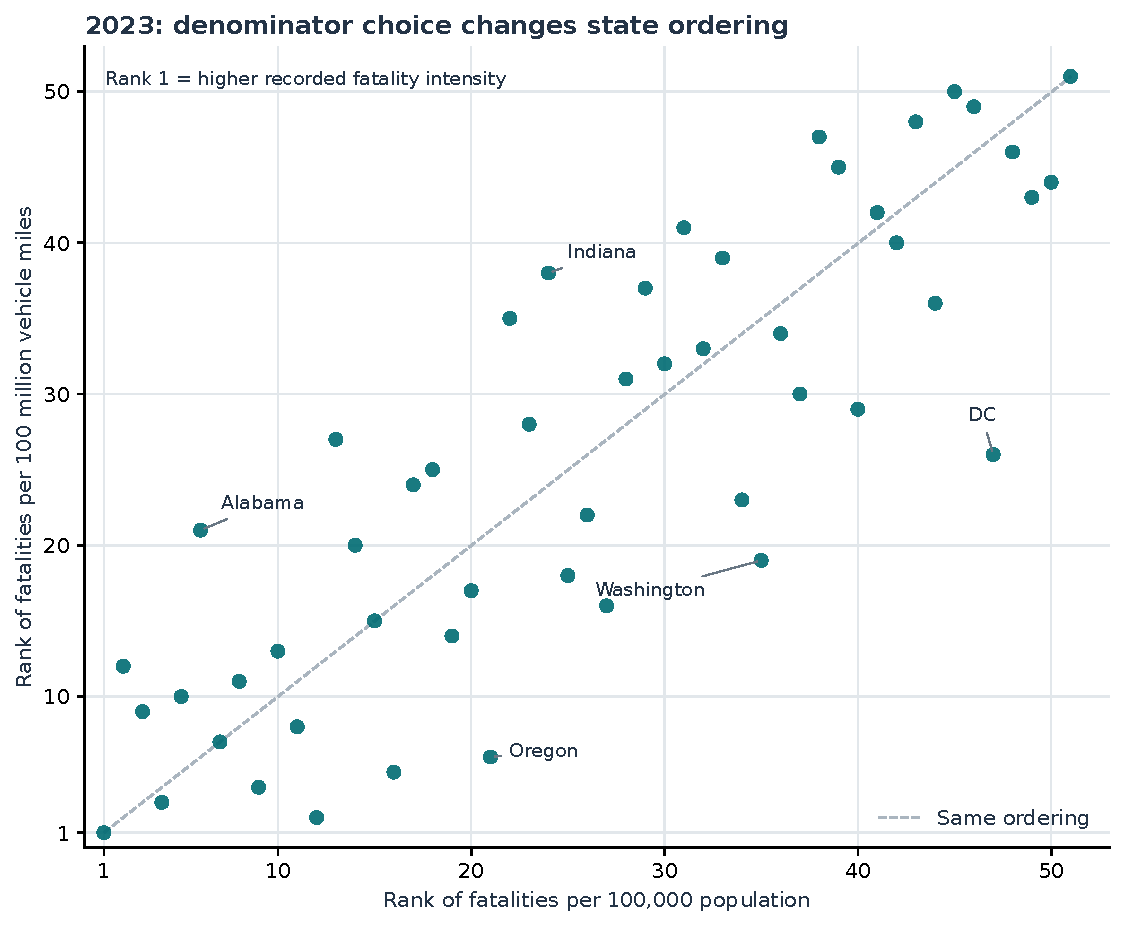
\includegraphics[width=.81\linewidth]{images/rank-scatter.pdf}\end{center}
\textbf{Figure 1.} All 51 states/DC under population and VMT denominators in the 2023 published snapshot. The diagonal denotes equal rank; each point is a state. Labels follow the fixed five-largest-absolute-movements rule, with alphabetical tie breaking. Full state-level rates, midranks and shortlist memberships are retained. The visual compares measures and does not identify safer states or causal mechanisms.

\begin{center}\begin{tabular}{lrrr}\toprule
State & Population rank & VMT rank & VMT minus population\\\midrule
District of Columbia & 47 & 26 & -21 \\
Washington & 35 & 19 & -16 \\
Alabama & 6 & 21 & +15 \\
Oregon & 21 & 6 & -15 \\
Indiana & 24 & 38 & +14 \\
\bottomrule\end{tabular}\end{center}
\textbf{Table 1.} The same fixed five annotated movements. A negative change moves toward higher recorded fatality intensity under VMT. These are descriptive rank changes, not estimates of individual traveler risk, residence-based mortality or an intervention effect.

\clearpage
\section*{4. Complete all-fatality contrasts}
Every denominator pair shows reversals in each report-year snapshot. We do not interpret the larger count of reversals in a later report as a causal or harmonized safety trend: each report retains its own ARF and denominator vintage.

\begin{center}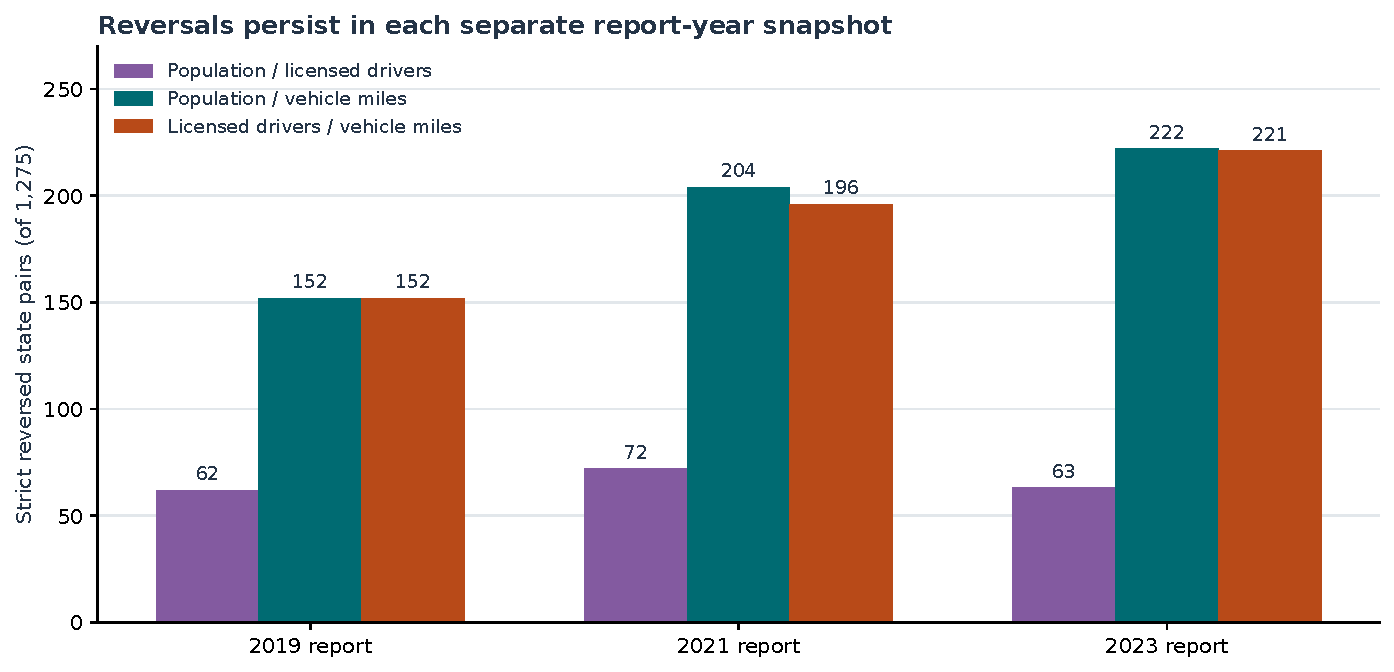
\includegraphics[width=\linewidth]{images/exact-reversals.pdf}\end{center}
\textbf{Figure 2.} Strict pair reversals for all fixed years and denominator contrasts, out of 1,275 state pairs in each bar. Zero is the count baseline. The underlying complete pair tables retain agreements and exact ties. No candidate contrast was omitted because its result was small.

\begin{center}\small\begin{tabular}{llrrrr}\toprule
Year & Denominator contrast & Reversals & Max move & Top5 overlap & Top10 overlap\\\midrule
2019 & Population / Licensed drivers & 62 & 8 & 4 & 9 \\
2019 & Population / Vehicle miles & 152 & 14 & 4 & 7 \\
2019 & Licensed drivers / Vehicle miles & 152 & 15 & 4 & 7 \\
2021 & Population / Licensed drivers & 72 & 8 & 4 & 9 \\
2021 & Population / Vehicle miles & 204 & 32 & 4 & 7 \\
2021 & Licensed drivers / Vehicle miles & 196 & 32 & 4 & 8 \\
2023 & Population / Licensed drivers & 63 & 7 & 3 & 9 \\
2023 & Population / Vehicle miles & 222 & 21 & 2 & 6 \\
2023 & Licensed drivers / Vehicle miles & 221 & 24 & 2 & 7 \\
\bottomrule\end{tabular}\end{center}
\textbf{Table 2.} All nine all-fatality contrasts. Max move is the largest absolute midrank movement. Every top-five and top-ten set has exactly five and ten states respectively in these runs. No tie is broken to force a fixed set size; the executable rule would retain all boundary ties.

The population/licensed-driver contrast has fewer reversals than either VMT contrast in each of these three snapshots. That pattern does not make the former a preferred measure: the appropriate denominator follows the question and the available exposure data. Neither population nor licensed-driver totals replace person-distance for nonmotorists.

\clearpage
\section*{5. Rounded shares and the fair exact-count comparator}
The selected 2019/2021 person-type tables supply whole percentages; their count ranges are necessary for analyses using only those cells. The 2023 table supplies exact counts, so its rounded-share representation is explicitly a coarsening sensitivity. The study retains the exact comparator rather than treating precision lost by display as missing source evidence.

\begin{center}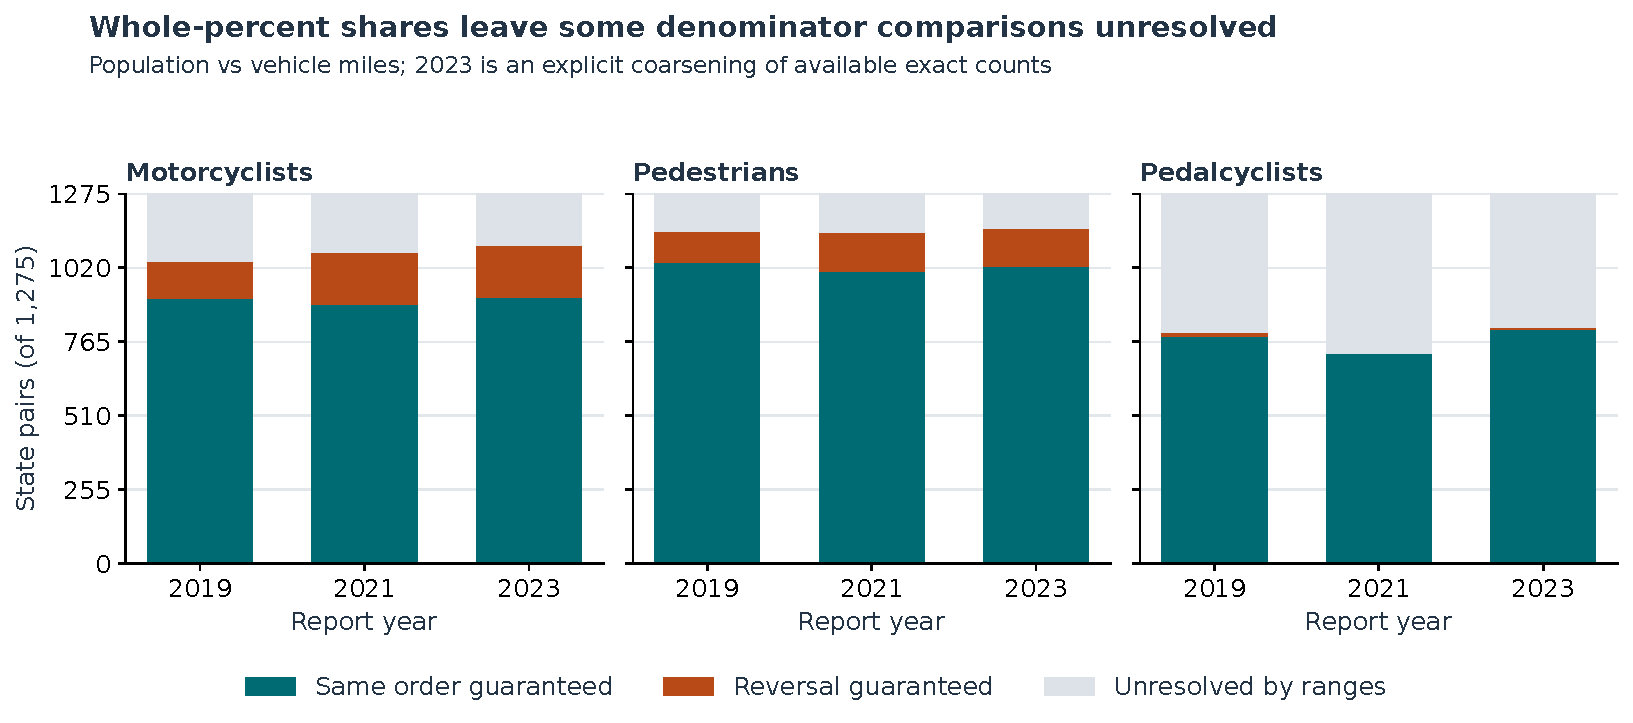
\includegraphics[width=\linewidth]{images/rounded-share-information.pdf}\end{center}
\textbf{Figure 3.} Population versus VMT pair classifications under closed percentage-count ranges and the fixed VMT display-precision sensitivity. Each bar totals 1,275 pairs. Guaranteed categories are sufficient conditional claims; unresolved includes overlap and ties. Year-specific person-type labels are preserved. The 2023 coarsening is compared with supplied exact counts below; bars are not pooled subgroup trends.

\begin{center}\small\begin{tabular}{lrrrrr}\toprule
2023 group & Exact reversals & Guaranteed & Unresolved & Reversals in unresolved & Exact ties\\\midrule
Motorcyclists & 262 & 180 & 179 & 82 & 0 \\
Pedestrians & 186 & 128 & 121 & 58 & 0 \\
Pedalcyclists & 126 & 7 & 461 & 119 & 6 \\
\bottomrule\end{tabular}\end{center}
\textbf{Table 3.} Primary population/VMT subgroup contrast. Guaranteed counts are from ranges; exact reversals/ties use supplied counts and printed denominator points. Every conditional guarantee agrees with the exact comparator, and every exact state midrank lies within its ordinal-placement range. All three denominator contrasts, exact point ranks/pairs, conditional ranges and contingency tables are retained.

For pedalcyclists, 461 pairs are unresolved by the ranges; they include 119 of the 126 exact strict reversals. The remaining seven reversals are guaranteed. This is information lost by the specified coarsening, not a measured error rate of an estimator. For motorcyclists, 262 exact reversals compare with 180 guaranteed; for pedestrians, 186 compare with 128. Use available exact counts and preserve the classification meaning before interpreting a rate.

\clearpage
\section*{6. Interpretation, limitations and next evidence}
\textbf{Label the measure before ranking it.} A comparison should display the recorded count, geographic event basis, denominator, unit, vintage and source precision together. Population-based intensity may be relevant to a broad geographic burden question; vehicle-mile intensity describes a different relationship to motor-vehicle travel. Neither is a complete basis for judging individual safety or deciding intervention priorities.

\textbf{Preserve precision.} Do not convert a rounded percentage to a point fatality count. Use exact subgroup counts when the source supplies them, as it does for the selected 2023 table. Where only rounded shares are available, retain feasible ranges and state which orderings are guaranteed versus unresolved. The conservative interval method is sufficient, not an exact joint enumeration of every feasible ranking.

\textbf{Keep years distinct.} FARS is a census of fatal motor-vehicle traffic crashes under its published inclusion rules [4]. These report snapshots retain ARF counts of 36,096, 42,939 and 40,901; later data releases may differ. The study does not estimate reporting-revision effects. NHTSA documents changes to vehicle classification from 2020 and motorized-bicycle classification from 2022 [5]. We preserve each year's labels and do not assert harmonized subgroup trends across those changes.

\textbf{The numerator and denominator can describe different populations.} Fatalities occur in a jurisdiction and may involve residents of other states. Population-based rates are therefore not resident mortality risks. Licensed drivers omit nondrivers and do not measure time or distance traveled. Total motor-vehicle VMT is not pedestrian/cyclist person-distance, nor motorcycle-specific mileage. Source estimates may have errors or revisions beyond printed rounding. No chosen range covers that broader uncertainty.

\textbf{No causal or operational claim.} State differences may reflect travel mix, road environment, reporting and many other factors not adjusted here. No model predicts an individual's injury, estimates an intervention effect, classifies legal compliance, or demonstrates safer travel, adopted policy, deployed users or realized savings. The fixed top-five/top-ten sets are measurement illustrations, not recommended allocations.

The next useful evidence is consistent road-user-specific distance or time exposure, auditable source vintages and classification crosswalks. A policy evaluation would additionally need a defined intervention, decision costs and a defensible causal design. A finer uncertainty analysis could enumerate coupled feasible counts or incorporate source estimation uncertainty when its distribution is available. None of those unexecuted extensions is claimed here.

\textbf{Contribution and authorship limits.} NHTSA already publishes multiple fatality-rate denominators side by side. This independent, AI-assisted work contributes a bounded reproducible comparison and explicit precision accounting using established arithmetic and ranking methods. It is not an exhaustive prior-work review, a new estimator, human-audited person-level label study, peer-reviewed paper or formal publication submission.

\clearpage
\section*{7. Reproduction and independent checks}
\begin{tabularx}{\linewidth}{l>{\raggedright\arraybackslash}X}\toprule
Gate & Current evidence\\\midrule
Source and coverage & 153 state-year rows; 1,872 fixed numeric source checks; 3,498 selected cells/locators independently matched by pypdf versus pdfplumber/pdfminer; six source-table pages inspected.\\
Boundaries & 13 fixtures cover closed rounding endpoints, zero/100\% shares, impossible cells/partitions, midrank ties, shortlist boundary ties and interval placement/dominance.\\
Independent arithmetic & 127,530 development and 63,765 evaluation values; 72,126 additional exact-subgroup comparator/containment checks. All required integer/rational equalities pass; displayed ratios have zero observed difference.\\
Isolated replay & 653,886 exact fields/JSON documents and 5,517 floating fields rebuilt offline; nineteen canonical dependencies verified.\\
Presentation & All 138 plotted values independently checked; three original figures and every manuscript page rendered for visual inspection.\\\bottomrule
\end{tabularx}

SQLite integer cross-products independently reconstruct midranks. Separate source-token joins, decimal ceiling/floor bounds and integer comparisons reconstruct rates, pair categories, contingency totals and placements. Exact values require equality; $10^{-12}$ absolute tolerance applies only to float display. Finite passing checks are not universal correctness, privacy, accessibility or scientific-novelty certification. Source failures and the prospective schema update remain in the record.

With Python 3.10 and pinned requirements:
\begin{verbatim}
python -m pip install -r requirements.txt
python -m unittest discover -s tests -v
python src/check_reproduction.py
python src/verify_figures.py
python src/verify_paper.py
python src/verify_public_package.py
\end{verbatim}
Public replay uses selected factual cells, with no PDF or live network required. Full-source verification additionally uses requirements-source.txt and excluded captured PDFs. Package checks bind reviewed canonical Git blobs and approved independent manuscript hashes. Remote Linux/merge/tree/tag proof is retained in the program register after verification. Separate formal-publication projects, including Azure optimization, remain private.

\section*{Primary references}
\small
[1] NHTSA (2021). \href{https://crashstats.nhtsa.dot.gov/Api/Public/ViewPublication/813183}{2019 State Traffic Data}, DOT HS 813 183, Tables 1 and 7.\par
[2] NHTSA (2023). \href{https://crashstats.nhtsa.dot.gov/Api/Public/ViewPublication/813509}{2021 State Traffic Data}, DOT HS 813 509, Tables 1 and 7.\par
[3] NHTSA (2025). \href{https://crashstats.nhtsa.dot.gov/Api/Public/ViewPublication/813743}{2023 State Traffic Data}, DOT HS 813 743, Tables 1 and 7.\par
[4] NHTSA, \href{https://www.nhtsa.gov/research-data/fatality-analysis-reporting-system-fars}{Fatality Analysis Reporting System}. Nationwide census and access/documentation.\par
[5] NHTSA, \href{https://www-fars.nhtsa.dot.gov/Help/helplinks.aspx}{FARS classification and file-version help}. Year-specific classification cautions.\par
[6] U.S. Copyright Office, \href{https://www.copyright.gov/what-is-copyright/}{What is copyright?} Facts versus protected expression. Reports attributed; complete report expression and registration fields excluded. All sources accessed 29 October 2026.
\end{document}
